
\documentclass[12pt,a4paper]{report}
\usepackage[utf8]{inputenc}
\usepackage{amsfonts}
\usepackage{setspace}
\usepackage{graphicx}
\usepackage{array}
\usepackage{fancyhdr}
\linespread{1.5}
\usepackage{geometry}
\geometry{
a4paper,
total={210mm,297mm},
left=1.25in,
right=0.75in,
top=0.75in,
bottom=0.75in,
}

\begin{document}
\pagestyle{empty}
\begin{center}
{\large \textbf{VISVESVARAYA TECHNOLOGICAL UNIVERSITY}}
\par
\vspace{3pt}
{\large \textbf{``JNANA SANGAMA'', BELAGAVI - 590 018}}
\begin{figure}[hbtp]
\centering

\includegraphics[width=0.80in,height=0.75in]{../fig/vtu}
\end{figure}
\\
\textbf{A MINI PROJECT REPORT}
\par
\textbf{on}
\par
\vspace{3pt}
{\Large \textbf{``GROCERY DELIVERY SYSTEM''}}
\par
\vspace{8pt}
\textit{\textbf{Submitted by}}
\par
\vspace{6pt}
\textbf{\large Akhilesh M             }\hspace{2.1in}\textbf{\large 4SF18IS008}\\
\textbf{\large Amaan Mohammad}\hspace{1.4in}\textbf{\large 4SF18IS010}\\
\par
\vspace{3pt}
\textit{\textbf{In partial fulfillment of the requirements for the V semester }}
\par
\vspace{0.5pt}
\Large \textbf{DBMS LABORATORY WITH MINI PROJECT}
\par
\vspace{0.5pt}
\normalsize \centering \textbf{of}
\par
\vspace{0.5pt}
\large \textbf{BACHELOR OF ENGINEERING }
\par
\vspace{0.5pt}
\textbf{in}
\par
\vspace{0.5pt}
\large \textbf{INFORMATION SCIENCE \& ENGINEERING}
\par
\vspace{2pt}
\textit{\textbf{Under the Guidance of}}
\par
\vspace{6pt}
\textbf{\large Mr. Rithesh Pakkala P.}\\
\normalsize\textbf{ Assistant Professor}\\
\normalsize\textbf{Department of ISE}\\
\par
\vspace{0.5pt}
\normalsize \centering \textbf{at}\\
\begin{figure}[hbtp]
\centering

\includegraphics[width=1.0in,height=0.85in]{../fig/registered}
\end{figure}
{\LARGE \textbf{SAHYADRI}}
\par
\vspace{6pt}
{\large \textbf{College of Engineering \& Management}}
\par
\vspace{3pt}
{\large \textbf{Adyar, Mangaluru - 575 007}}
\par
\vspace{3pt}
{\large \textbf{2020 - 21}}

\newpage

{\LARGE \textbf{SAHYADRI}}
\par
\vspace{6pt}
{\Large \textbf{College of Engineering \& Management}}
\par
\vspace{3pt}
{\large \textbf{Adyar, Mangaluru - 575 007}}
\par
\vspace{0.25in}
{\large \textbf{Department of Information Science \& Engineering}}
\par
\begin{figure}[hbtp]
\centering

\includegraphics[width=1.0in,height=0.75in]{../fig/registered}
\end{figure}
{\Large \textbf{CERTIFICATE}}
\end{center}
\par
\vspace{0.10in}
\setstretch{1.5}
\noindent This is to certify that the \textbf{Mini Project} entitled \textbf{``Grocery   Delivery   System''}  has been carried out by 
\textbf{Akhilesh M (4SF18IS008)} and ,\textbf{ Amaan Mohammad (4SF18IS010)} the bonafide students of Sahyadri College of Engineering \& Management in partial fulfillment of the requirements for the V semester \textbf{DBMS Laboratory with Mini Project (18CSL58)} of \textbf{Bachelor of Engineering in Information Science \& Engineering} of Visvesvaraya Technological University, Belagavi during the year  2020 - 21. It is certified that all corrections/suggestions indicated for Internal Assessment have been incorporated in the report deposited in the departmental library. The mini project report has been approved as it satisfies the academic requirements in respect of mini project work.

\par
\vspace{0.75in}
\setstretch{1.15}
\begin{tabbing}
-----------------------------------\hspace{2.5in}\=---------------------------------\\
\textbf{Mr. Rithesh Pakkala P.}\>\hspace{0.2in}\textbf{Dr. Shamanth Rai}\\
\hspace{0.30in}Assistant Professor\>\hspace{0.001in}HOD \& Associate Professor\\
\hspace{0.21in}Dept. of ISE, SCEM\>\hspace{0.2in}Dept. of ISE, SCEM\\

\end{tabbing}

\par
\vspace{0.25in}
\begin{center}
\large \textbf{External Practical Examination:}
\end{center}
\begin{flushleft}
\begin{normalsize}Examiner's Name \end{normalsize}
\hspace{7.5cm}
\begin{normalsize}Signature with Date\end{normalsize}
\end{flushleft}
\par
\vspace{0.05in}
\begin{flushleft}
1. \ldots\ldots\ldots\ldots\ldots\ldots \ldots \hspace{6.8cm}\ldots\ldots\ldots\ldots \ldots\ldots\ldots 
\par
\vspace{0.25in}	
2. \ldots\ldots\ldots\ldots\ldots\ldots \ldots \hspace{6.8cm}\ldots\ldots\ldots\ldots \ldots\ldots\ldots 
\end{flushleft}


\newpage
\begin{center}
{\LARGE \textbf{SAHYADRI}}
\par
\vspace{6pt}
{\Large \textbf{College of Engineering \& Management}}
\par
\vspace{3pt}
{\large \textbf{Adyar, Mangaluru - 575 007}}
\par
\vspace{0.25in}
{\large \textbf{Department of Information Science \& Engineering}}
\par
\begin{figure}[hbtp]
\centering

\includegraphics[width=1.25in,height=1in]{../fig/registered}
\end{figure}
{\Large \textbf{DECLARATION}} 
\end{center}
\par
\vspace{0.10in}
\setstretch{1.5}
\noindent We hereby declare that the entire work embodied in this Mini Project Report titled
\textbf{``Grocery Delivery System''} has been carried out by us at Sahyadri College of Engineering and Management, Mangaluru under the supervision of \textbf{Mr. Rithesh Pakkala P.} as the part of the V semester \textbf{DBMS Laboratory with Mini Project (18CSL58)} of \textbf{Bachelor of Engineering} in \textbf{Information Science \& Engineering}. This report has not been submitted to this or any other University.\\
\vspace{0.25in}
\begin{flushright}
\textbf{Akhilesh M (4SF18IS008)}\\
\textbf{Amaan Mohammad (4SF18IS010)}\\
SCEM, Mangaluru \\
\end{flushright}

% For Individuals
%\begin{flushright}
%Place: Mangaluru \hspace{7.8cm} \textbf{Student Name 1}\\
%Date : \hspace{11.7cm}4SF11IS001\\
%V Semester, B.E., ISE\\
%SCEM, Mangaluru\\
%\end{flushright}

\newpage
\pagestyle{plain}
\pagenumbering{roman}
\chapter*{Abstract}
\addcontentsline{toc}{chapter}{\numberline{}Abstract}
Helpy Hands is a startup where we specialize in groceries and essentials 
delivery to the customers doorstep. In this project we have highlighted the behind the scenes process. To improve 
the experience of both the customer, seller and the delivery agent our comprehensive database specializes in quick 
real-time updation of Customer details , Shop stocks and delivery agent availability and tracking. All these 
elements work seamlessly from when the order is placed from the customer side right through the Shop's inventory 
and the order tracking of the customer.
\chapter*{Acknowledgement}
\addcontentsline{toc}{chapter}{\numberline{}Acknowledgement}
It is with great satisfaction and euphoria that we are submitting the Mini Project Report on \textbf{“Grocery Delivery System”}. We have completed it as a part of the V semester \textbf{DBMS Laboratory with Mini Project (18CSL58)} of \textbf{Bachelor of Engineering} in \textbf{Information Science \& Engineering} of Visvesvaraya Technological University, Belagavi.
\par
\vspace{0.15in}
\noindent We are profoundly indebted to our guide, \textbf{Mr. Rithesh Pakkala P.}, Assistant Professor, Department of Information Science \& Engineering for innumerable acts of timely advice, encouragement and We sincerely express our gratitude.
\par
\vspace{0.15in}
\noindent We express our sincere gratitude to \textbf{Dr. Shamanth Rai}, Head \& Associate Professor, Department of Information Science \& Engineering for his invaluable support and guidance.
\par
\vspace{0.15in}
\noindent We sincerely thank  \textbf{Dr. Rajesha S}, Principal, Sahyadri College of Engineering \& Management  and \textbf{Dr. D. L. Prabhakara}, Director, Sahyadri Educational Institutions,who have always been a great source of inspiration.
\par
\vspace{0.15in}
\noindent Finally, yet importantly, We express our heartfelt thanks to our family \& friends for their wishes and encouragement throughout the work.
\\
\\
%\begin{flushright}
%\textbf{Student Name 1}\\
%\textbf{Student Name 2}\\
%\end{flushright}

% For Individuals
\begin{flushright}
\textbf{Akhilesh M}\hspace{6.7cm}\textbf{Amaan Mohammad}\\
\hspace{0.2in}4SF18IS008 \hspace{3.38in}4SF18IS010\\
V Sem, B.E., ISE\hspace{7.7cm}V Sem, B.E., ISE\\
SCEM, Mangaluru\hspace{7.5cm}SCEM, Mangaluru\\
\end{flushright}

\setstretch{1.3}
\renewcommand{\contentsname}{Table of Contents}
\tableofcontents
\addcontentsline{toc}{chapter}{\numberline{}Table of Contents}
\listoffigures
\addcontentsline{toc}{chapter}{\numberline{}List of Figures}
\newpage

\pagestyle{fancy}
\fancyhf{}
\lhead{\fontsize{10}{12} \selectfont Grocery Delivery System}
\rhead{\fontsize{10}{12} \selectfont Chapter \thechapter}
\lfoot{\fontsize{10}{12} \selectfont Department of Information Science \& Engineering, SCEM, Mangaluru}
\rfoot{\fontsize{10}{12} \selectfont Page \thepage}
\renewcommand{\headrulewidth}{0.5pt}
\renewcommand{\footrulewidth}{0.5pt}

\setstretch{1.5}
\pagenumbering{arabic}
\chapter{Introduction}

When the entire world was reeling from the effects of Covid-19 and lockdown, it was tough time for all of us to be locked inside our homes. There arised a problem of people having difficulties in shopping for food , essentials and medicines. Therefore we founded a start-up where it enabled anyone to order essentials or medicines from the shop of their choice and have it delivered to their home. This discouraged people from stepping outside which helped curb the spread of virus considerably. 
\section{Database Management System }

With the widespread use of computer technology and network technology, the development of database technology has become an important part of advanced information technology. The core of the supermarket management system is how to use and operate database, so the database design is critical. This system uses the Oracle10g database which is a relational database management system of Oracle. It is a product that always has been a leading position in the field of database. The Oracle database system is the world popular relational database management system which easy to use, strong function and suitable for all kinds of large, medium and small, microcomputer environment. It can realize data sharing and the facilities don't need to have the powerful data storage and processing capabilities so that to reduce the hardware cost of supermarket. Many enterprises have their own database, and store a large number of key data in it, which shows the importance of the database.\\
Every table in the database is broken up into smaller entities called fields. The fields in the Customers table consist of CstID, CstName ,CstPhoneNo ,  CstEmail A field is a column in a table that is designed to maintain specific information about every record in the table. A record, also called a row, is each individual entry that exists in a table. A record is a horizontal entity in a table. A column is a vertical entity in a table that contains all information associated with a specific field in a table. In addition to tables, a database can also contain other objects including views, stored procedures, indexes and constraints, along with a transaction log.


\section{Structured Query Language}

SQL is a domain specific language used in programming  and designed for managing data held in a database management system. SQL consists of a data definition language, data manipulation language and data control language. The scope of SQL includes data insert, query update and delete, schema creation and modification and data access control. As a database server, it is a software product with the primary function of storing and retrieving data as requested by other software applications which may run either on the same computer or on another computer across a network.
The main mode of retrieving data from a SQL Server database is querying for it. The query declaratively specifies what is to be retrieved. It is processed by the query processor, which figures out the sequence of steps that will be necessary to retrieve the requested data. The sequence of actions necessary to execute a query is called a query plan. There might be multiple ways to process the same query.Stored procedures can accept values sent by the client as input parameters, and send back results as output parameters. They can call defined functions, and other stored procedures, including the same stored procedure.

\section{Stored Procedure}
A stored procedure is a prepared SQL code that you can save, so the code can be reused over and over again.
So if you have an SQL query that you write over and over again, save it as a stored procedure, and then just call it to execute it.We can also pass parameters to a stored procedure, so that the stored procedure can act based on the parameter value(s) that is passed.A stored procedure is nothing more than prepared SQL code that you save so you can reuse the code over and over again.  So if you think about a query that you write over and over again, instead of having to write that query each time you would save it as a stored procedure and then just call the stored procedure to execute the SQL code that you saved as part of the stored procedure.In addition to running the same SQL code over and over again you also have the ability to pass parameters to the stored procedure, so depending on what the need is the stored procedure can act accordingly based on the parameter values that were passed.

\section{Normalisation}
Database Normalization is a technique of organizing the data in the database. Normalization is a systematic approach of decomposing tables to eliminate data redundancy(repetition) and undesirable characteristics like Insertion, Update and Deletion Anamolies. It is a multi-step process that puts data into tabular form, removing duplicated data from the relation tables.\\
Normalization is used for mainly two purposes:\\
1.Eliminating redundant(useless) data.\\
2.Ensuring data dependencies make sense i.e data is logically stored.

\section{Application}
This project enables customers to buy anything and everything from the comfort of their homes. Groceries , essentials and pretty much everything can be home delivered from nearby shops. Helps save fuel and money whilst also helping customers save time. This is especially usefull during the time of pandemics. It encourages people to stay home and limits the spread of virus.

\chapter{Hardware and Software Details}
\section{Hardware Details}
\begin{itemize}
\item Processor : Any Processor more than 500 MHz
\item RAM : 2GB
\item Hard Disk : 5GB
\item Input Device : Standard Keyboard and Mouse
\item Output Device : Monitor
\end{itemize}
\section{Software Details}
\begin{itemize}
\item Database : MySql
\item Programming Language : Python
\item IDE : Visual Studio Code
\item Operating System : Windows 10
\end{itemize}

\chapter{System Design}
\section{Entity Relation Diagram(ERD)}
\par
An entity relationship diagram (ERD) shows the relationships of entity sets stored in a database. An entity in this context is an object, a component of data. These entities can have attributes that define its properties. By defining the entities, their attributes, and showing the relationships between them, an ER diagram illustrates the logical structure of databases.\\
\begin{flushleft}
\textbf{ERD Entity Symbols:}\\
\end{flushleft}
\begin{flushleft}
Entities are objects or concepts that represent important data. Entities are typically nouns such as product, customer, location, or promotion.An entity is represented as rectangle in an ER diagram. There are three types of entities commonly used in entity relationship diagrams.\\
\end{flushleft}
\begin{figure}[hbtp]
\begin{center}
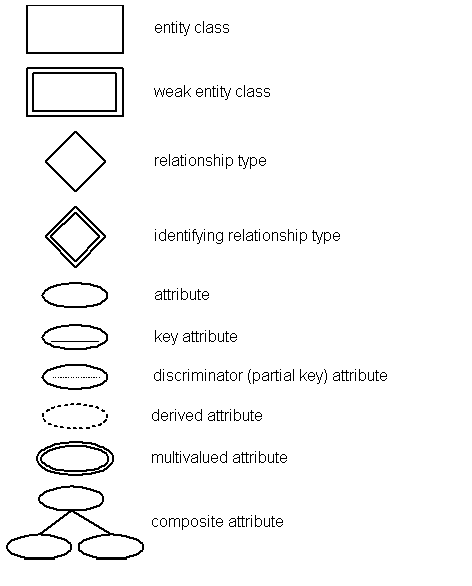
\includegraphics[width=6in,height=4in]{../fig/ERSYMBOLS}
\end{center}
\caption{ER Diagram Symbols }
\end{figure}
\begin{flushleft}
\textbf{Cardinality Ratios:}\\
\end{flushleft}
Cardinality refers to the maximum number of times an instance in one entity can relate to instances of another entity.\
\begin{figure}[hbtp]
\begin{center}
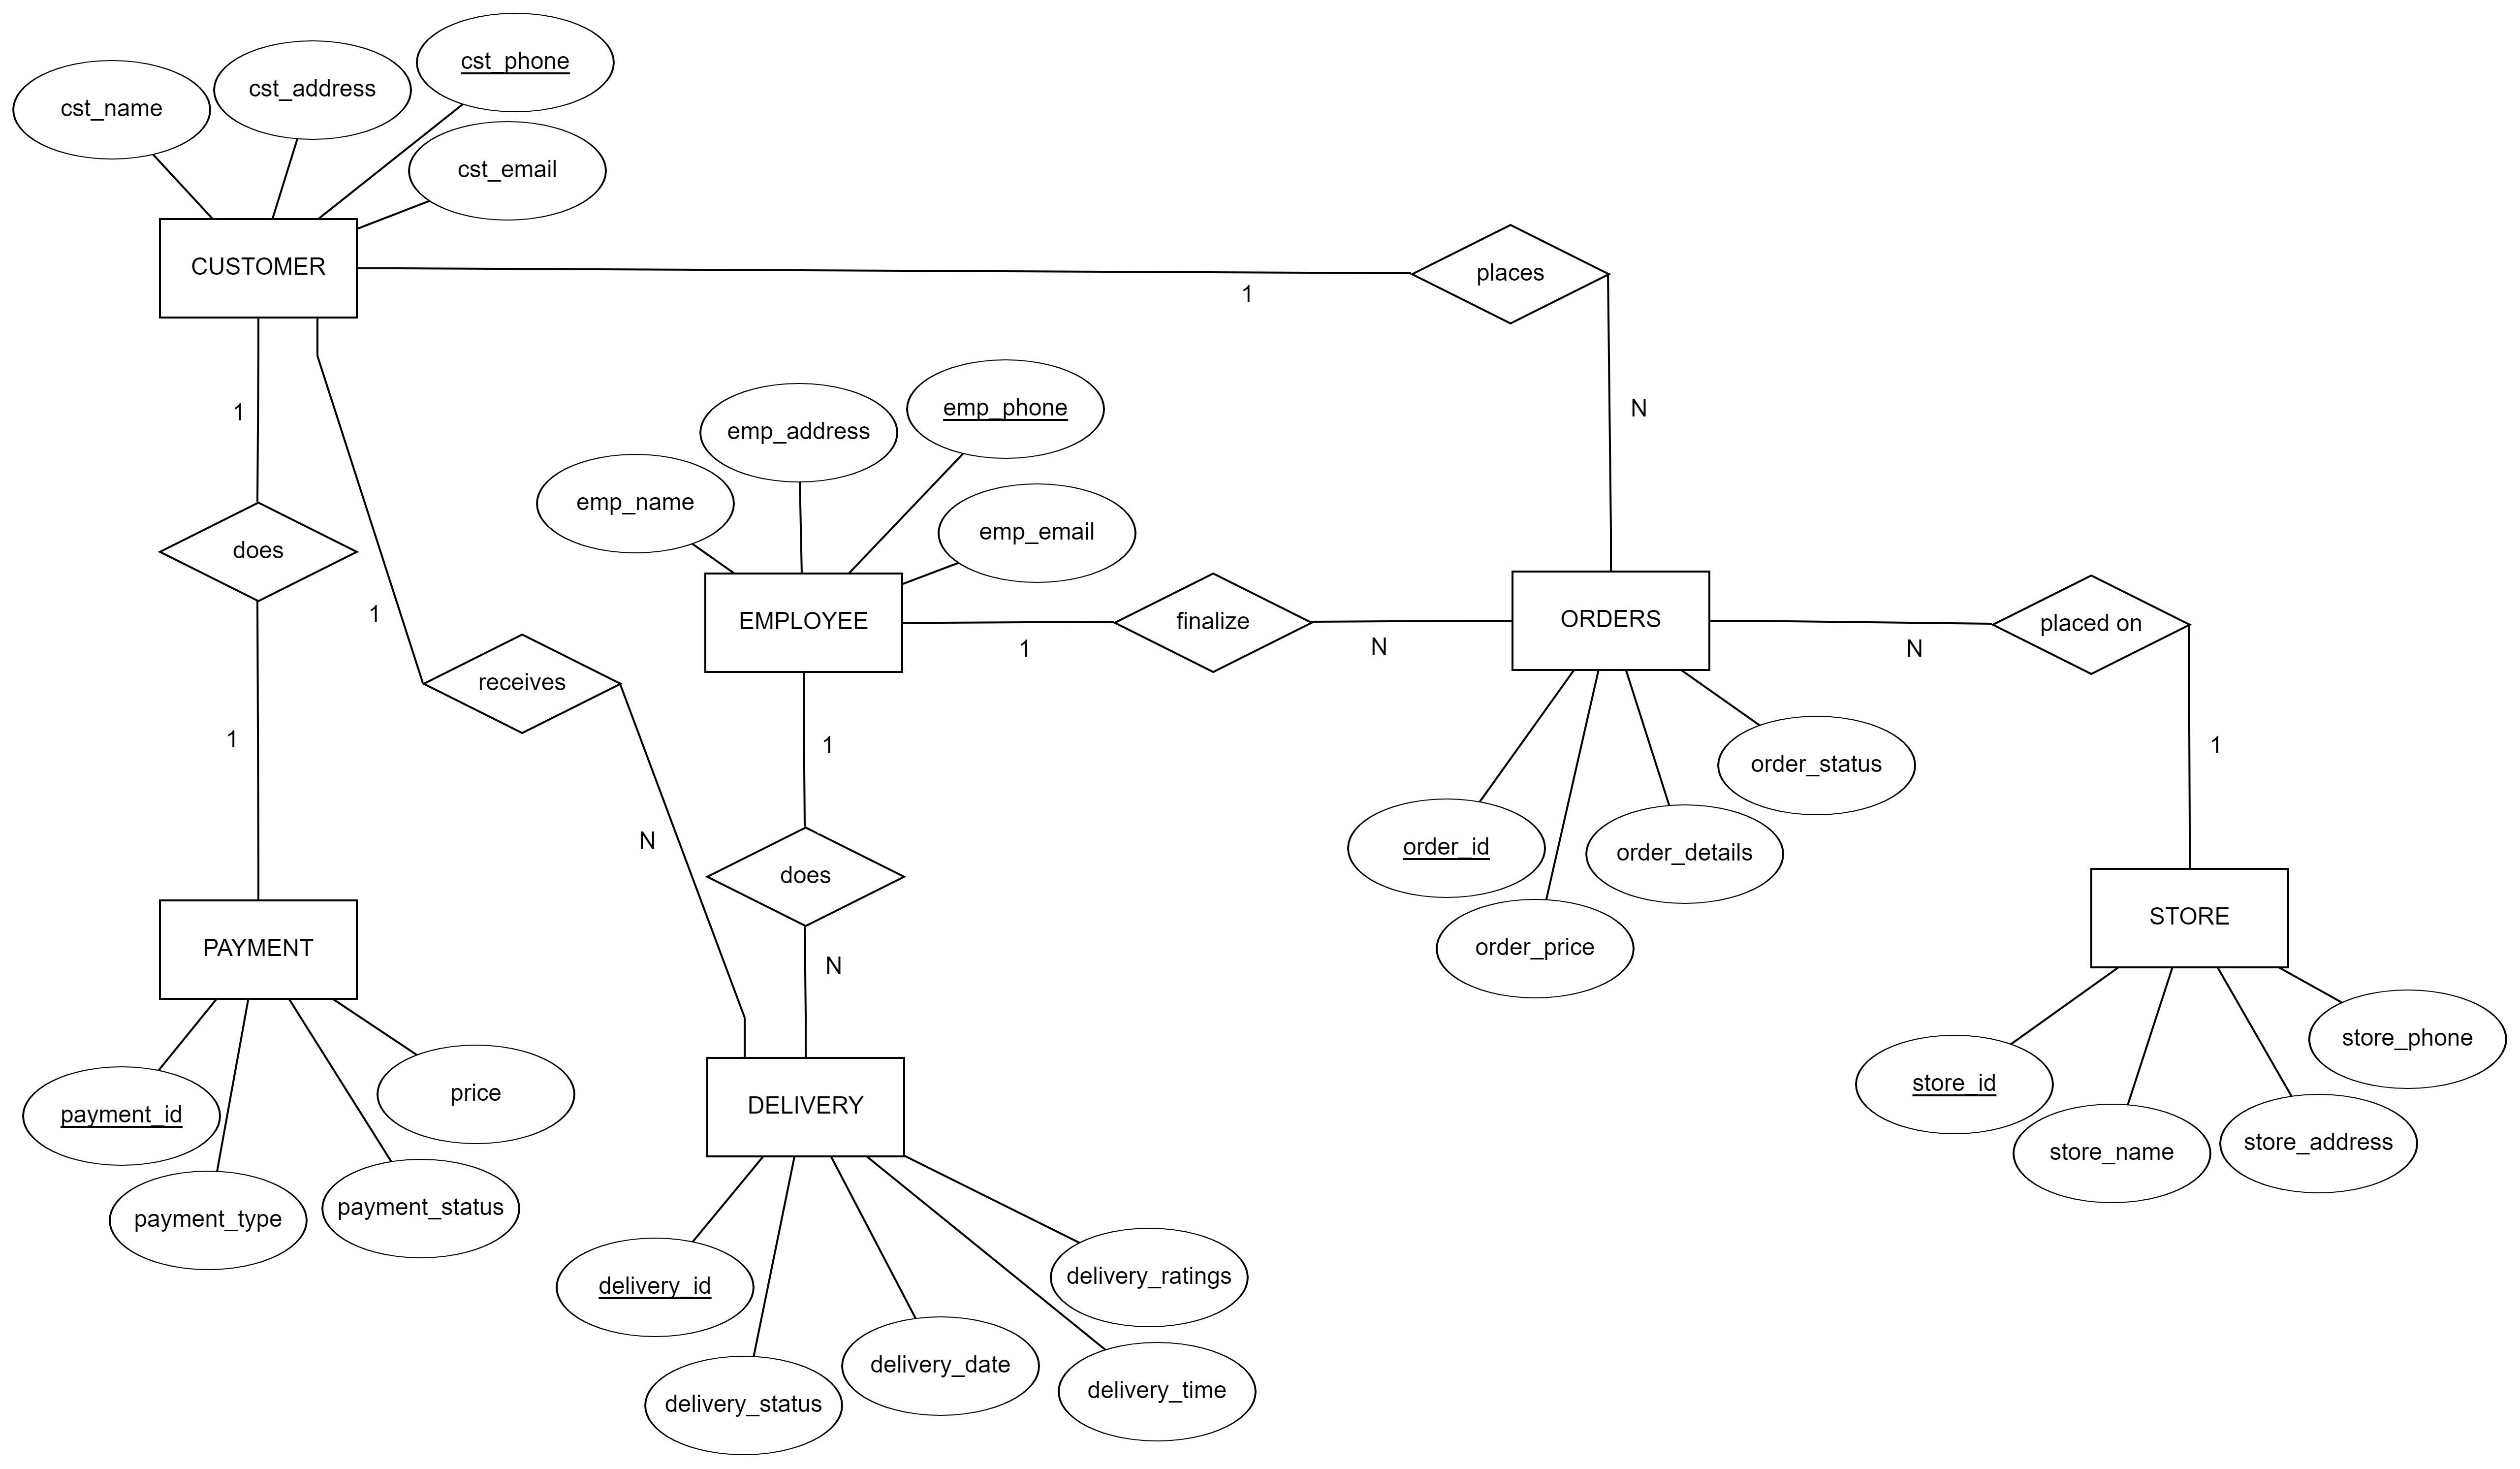
\includegraphics[width=6in,height=4in]{../fig/cardi}
\end{center}
\caption{ER Diagram Cardinality Ratios}
\end{figure}



\newpage
\section{Mapping From ER Diagram to Schema Diagram}
\textbf{1.Mapping of Regular Entities}:This step involves mapping all the regular entity types to tabular format by identifying their primary keys.\\
\textbf{2.Mapping of 1:1 Relation:}In this step foreign keys are assigned using foreign key approach.The primary key of the participating relation R or S is added as primary key to second entity types by looking at the participating constraints.\\
\textbf{3.Mapping of 1:N Relation:}Foreign key approach is used to add one sided primary key to the n sided entity at foreign key.\\
\textbf{4.Mapping of M:N Relation:}Here we use the cross reference approach where the relationship is converted to a new relation within attributes on primary keys of both participating relation.\\
\textbf{5.Mapping of Weak Entity:}When mapping weak entity types along with other attributes the partial key and primary key of parent entity together will form their primary key of the new relation.\\
\textbf{6.Mapping of N-ary Relation:}For mapping N array relationship we create a new relation with a relationship name in its attribute and primary keys of all participating entity types.\\
\textbf{7.Mapping of Multivalued Relation:}For multivalued attributes a separate relation has to be created along with primary key of parent relation.\\
In our database we have the following mappings:\\
\linebreak
\textbf{Step – 1 : Mapping of Regular Entities.}\\
For each regular (strong) entity type E in the ER schema, create a relation R that includes all the simple attributes of E. Include only the simple component attributes of a
composite attribute. Choose one of the key attributes of E as primary key for R. If the
chosen key of E is composite, the set of simple attributes that form it will together form
the primary key of R.\\
\begin{figure}[hbtp]
\centering
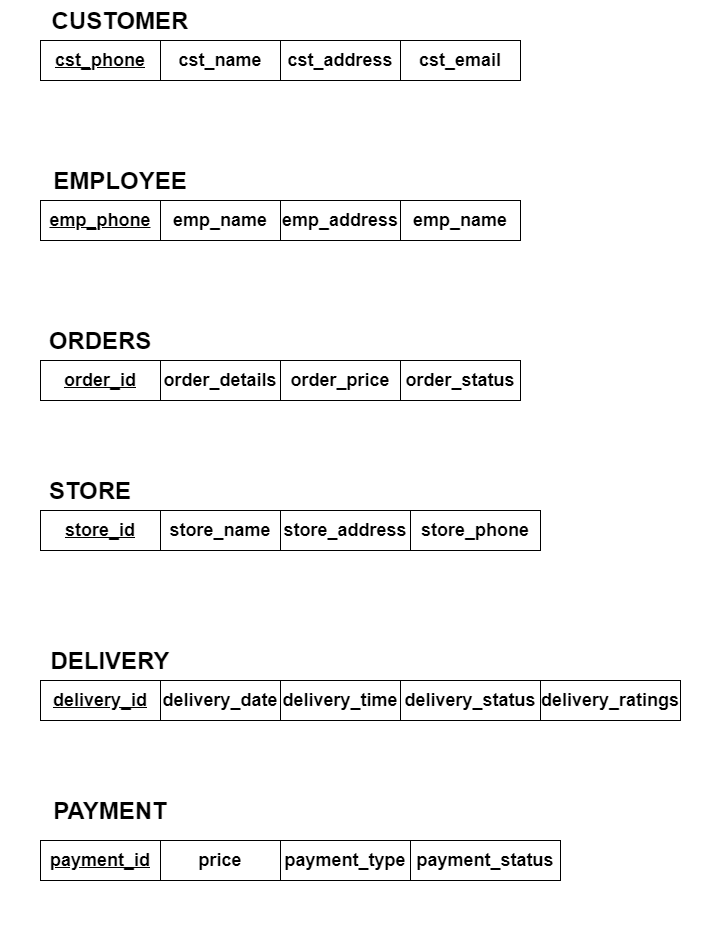
\includegraphics[width=6in,height=7in]{../fig/regular (1)}
\caption{Regular Entities}
\end{figure} 
\newpage
\noindent \textbf{Step – 2 : Mapping of binary 1:1 Relation Types.}\\
The Payment and the Customer entities are participating in the 1:1 relation type. Since Payment has a total participation in the relation we include the primary key of Customer entity as the foreign key in Payment entity.\\
\begin{figure}[hbtp]
\centering
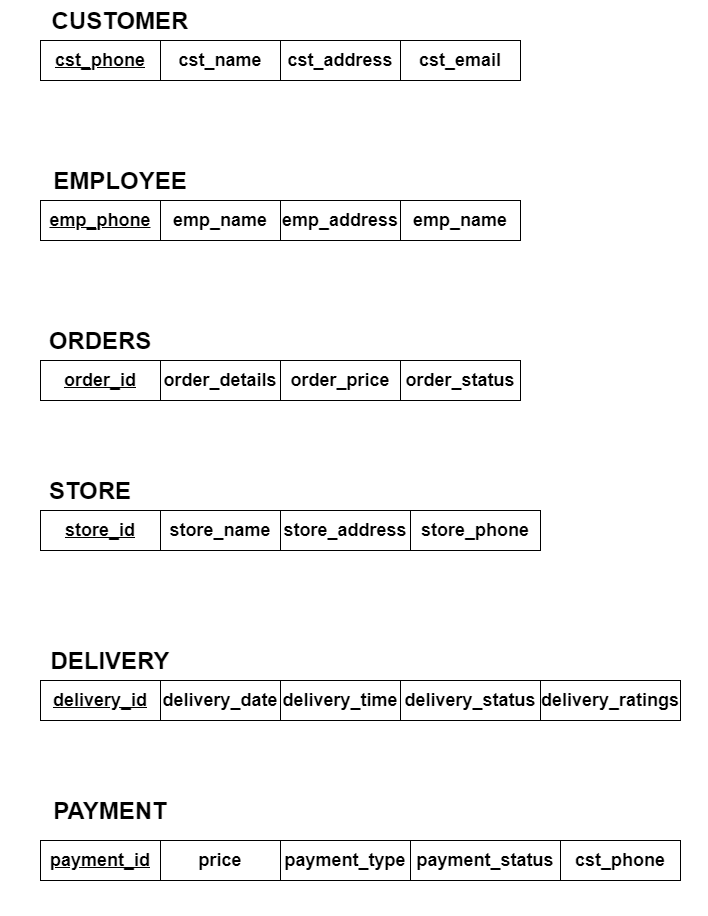
\includegraphics[width=6in,height=7in]{../fig/1to1 (1)}
\caption{1:1 Relations}
\end{figure} 
\newpage
\noindent\textbf{Step – 3 : Mapping of binary 1:N Relation Types.}\\
The Customer and the Order entities are participating in the 1:N relation type. Since Order in one the nth side of the relation we include the primary key of Customer entity as the Foreign key in Order entity.\\
The Employee and the Order entities are participating in the 1:N relation type. Since Order in one the nth side of the relation we include the primary key of Employee entity as the Foreign key in Order entity.\\
The Store and the Order entities are participating in the 1:N relation type. Since Order in one the nth side of the relation we include the primary key of Store entity as the Foreign key in Order entity.\\
The Employee and the Delivery entities are participating in the 1:N relation type. Since Delivery in one the nth side of the relation we include the primary key of Employee entity as the Foreign key in Delivery entity.\\
\begin{figure}[hbtp]
\centering
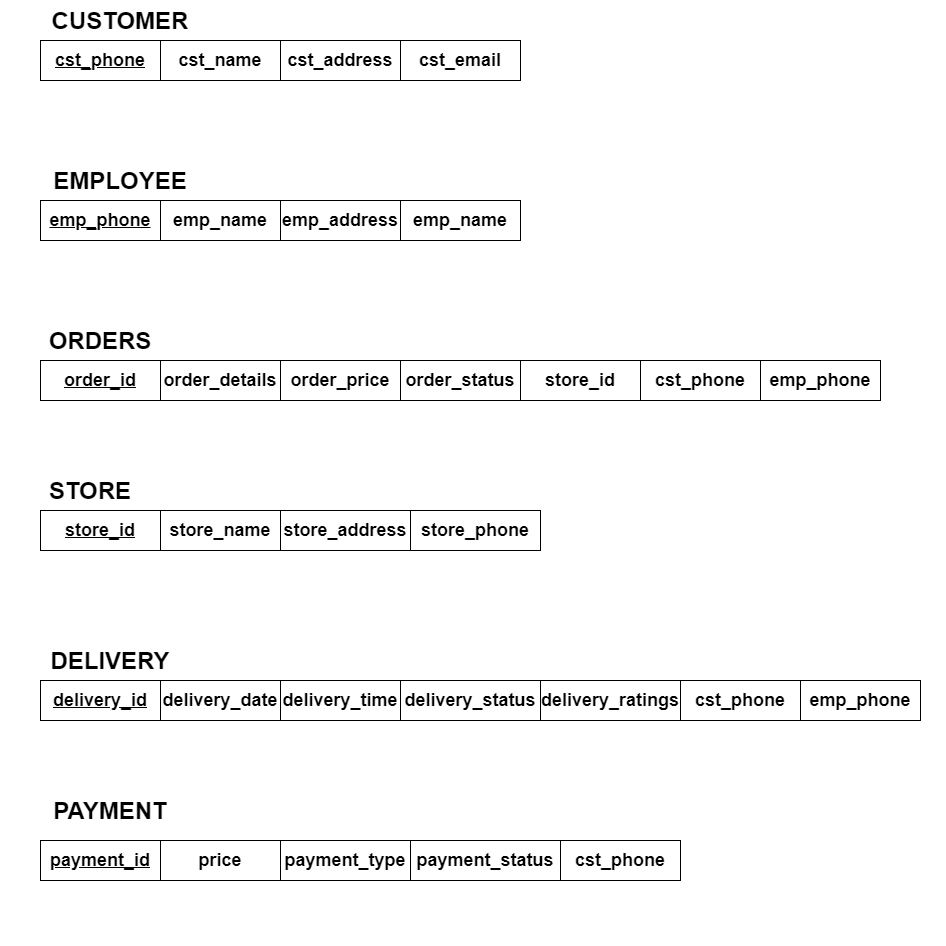
\includegraphics[width=6in,height=5in]{../fig/1toN (1)}
\caption{1:N Relations}
\end{figure} 
\newpage

\section{Schema Diagram}
\par
A Schema is a pictorial representation of the relationship between the database tables in the database that is created. The database schema of a database system is its structure described in a formal language sup ported by the database management system (DBMS). The term "schema" refers to the organization of data as a blueprint of how the database is constructed (divided into database tables in the case of relational databases). The formal definition of a database schema is a set of formulas (sentences) called integrity constraints imposed on a database. These integrity constraints ensure compatibility between parts of the schema. All constraints are expressible in the same language. A database can be considered a structure in realization of the database language.The states of a created conceptual schema are transformed into an explicit mapping, the database schema. This describes how real-world entities are modelled in the database.
\newpage
\begin{figure}[hbtp]
\centering
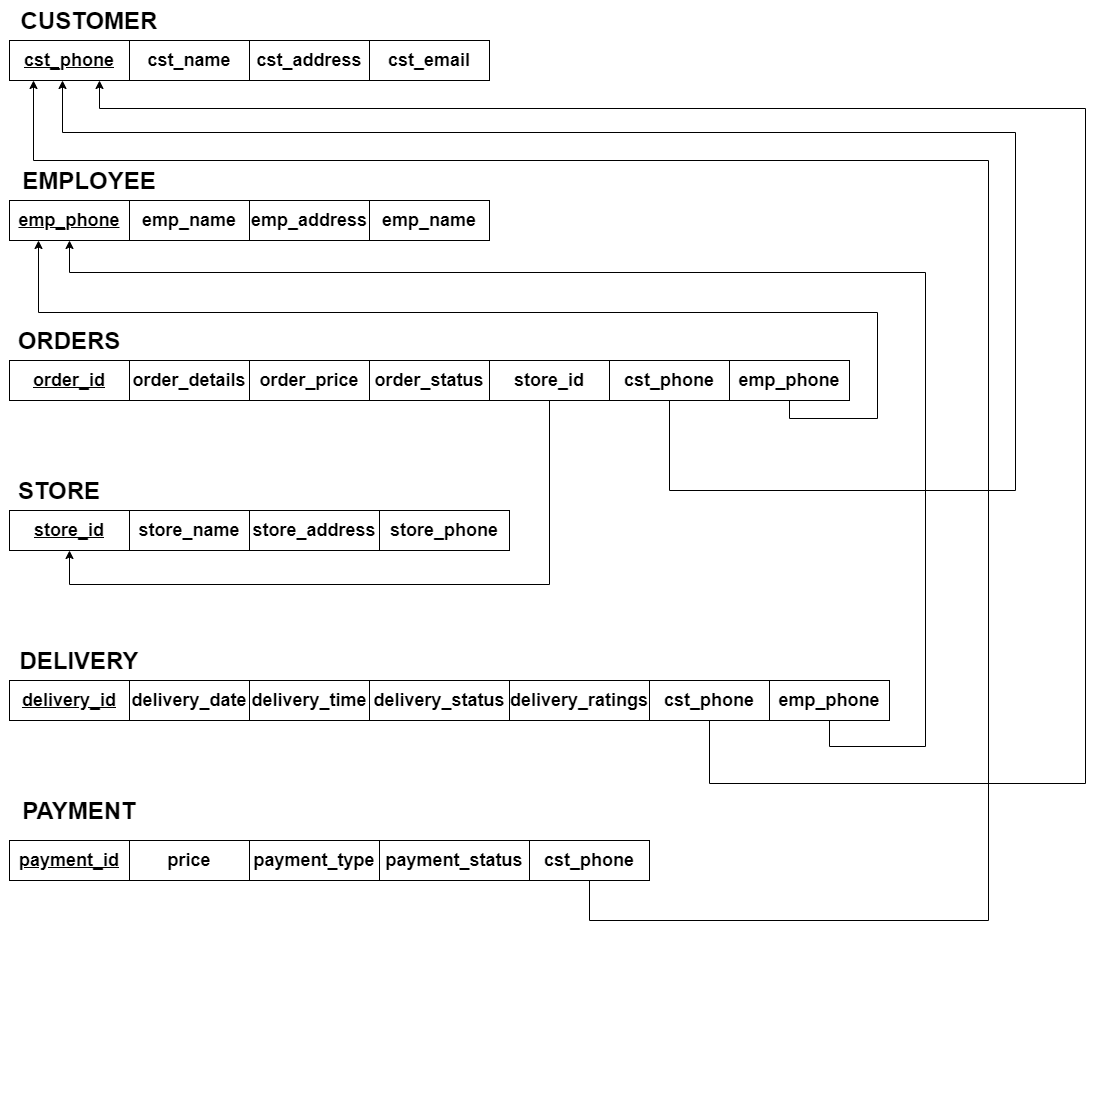
\includegraphics[width=6in,height=8in]{../fig/proper schema}
\caption{Schema Diagram Of Grocery Delivery System}
\end{figure}


\chapter{Implementation}
\section{Programming Languages Used}
\textbf{Python}\\
Python is an interpreted, high-level and general-purpose programming language usedworldwide. Python’s design philosophy emphasizes code readability with its notable useof significant white space.FlaskFlask is a micro web framework written in Python. It is classified as a micro-frameworkbecause it does not require particular tools or libraries. It has no database abstractionlayer, form validation, or any other components where pre-existing third-party librariesprovide common functions.Sqlite3SQLite is a relational database management system contained in a C library. In contrastto many other database management systems, SQLite is not a client–server databaseengine. Rather, it is embedded into the end program.\\
\linebreak
\textbf{Flask}\\
Flask is a micro web framework written in Python. It is classified as a micro-frameworkbecause it does not require particular tools or libraries. It has no database abstractionlayer, form validation, or any other components where pre-existing third-party librariesprovide common functions.\\
\linebreak
\textbf{SQLite3}\\
SQLite is a relational database management system contained in a C library. In contrastto many other database management systems, SQLite is not a client–server databaseengine. Rather, it is embedded into the end program.\\
\linebreak
\section{Table Structure}
\textbf{CUSTOMER}\\
\begin{figure}[hbtp]
\centering
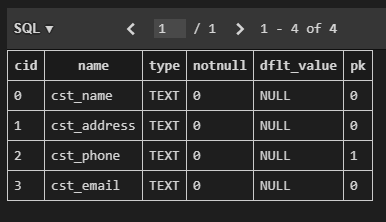
\includegraphics[width=5in,height=2in]{../fig/customer}\\
\end{figure}\\
CREATE TABLE IF NOT EXISTS CUSTOMER(\\
cst\_name TEXT,\\
cst\_address TEXT,\\
cst\_ phone TEXT PRIMARY KEY,\\
cst\_email TEXT );    \\
\linebreak
\textbf{EMPLOYEE}\\
\begin{figure}[hbtp]
\centering
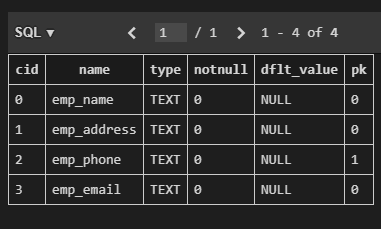
\includegraphics[width=5in,height=2in]{../fig/employee}\\
\end{figure}
\newpage
\noindent CREATE TABLE IF NOT EXISTS EMPLOYEE(\\
emp\_name TEXT,\\
emp\_address TEXT,\\
emp\_phone TEXT PRIMARY KEY,\\
emp\_email TEXT  );\\
\begin{flushleft}
\textbf{STORE}\\
\end{flushleft}
\begin{figure}[hbtp]
\centering
\includegraphics[width=5in,height=2in]{../fig/store}\\
\end{figure}
CREATE TABLE IF NOT EXISTS STORE(\\
 store\_id INTEGER PRIMARY KEY,\\
 store\_name TEXT,\\
 store\_address TEXT,\\
 store\_phone TEXT );\\
\begin{flushleft}
\textbf{ORDER}\\
\end{flushleft}
\begin{figure}[hbtp]
\centering
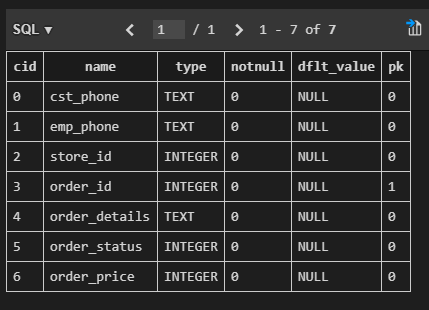
\includegraphics[width=5in,height=2in]{../fig/orders}\\
\end{figure}
CREATE TABLE IF NOT EXISTS ORDERS(\\
cst\_phone TEXT,\\
emp\_phone TEXT,\\
store\_id INTEGER,\\
order\_ id INTEGER PRIMARY KEY, \\
order\_details TEXT,\\
order\_status INTEGER,\\
order\_price INTEGER,\\
FOREIGN KEY(cst\_phone) REFERENCES CUSTOMER(cst\_phone) ON DELETE CASCADE,\\
FOREIGN KEY(emp\_phone) REFERENCES EMPLOYEE(emp\_phone) ON DELETE CASCADE,\\
FOREIGN KEY(store\_id) REFERENCES STORE(store\_id) ON DELETE CASCADE );\\
\begin{flushleft}
\textbf{DELIVERY}\\
\end{flushleft}
\begin{figure}[hbtp]
\centering
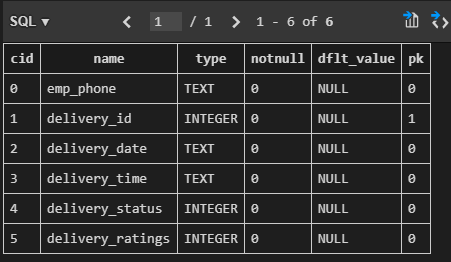
\includegraphics[width=5in,height=2in]{../fig/delivery}\\
\end{figure}
CREATE TABLE IF NOT EXISTS DELIVERY(\\
emp\_phone TEXT,\\
cst\_phone TEXT,\\
delivery\_id INTEGER PRIMARY KEY,\\
delivery\_date TEXT,\\
delivery\_time TEXT,\\
delivery\_status INTEGER,\\
delivery\_ratings INTEGER,\\
FOREIGN KEY(cst\_phone) REFERENCES CUSTOMER(cst\_phone) ON DELETE CASCADE,\\
FOREIGN KEY(emp\_phone) REFERENCES EMPLOYEE(emp\_phone) ON DELETE CASCADE );\\
\begin{flushleft}
\textbf{PAYMENT}\\
\end{flushleft}
\begin{figure}[hbtp]
\centering
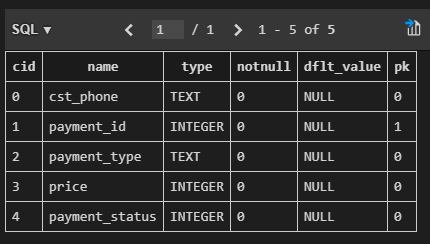
\includegraphics[width=5in,height=2in]{../fig/payment}
\end{figure}
CREATE TABLE IF NOT EXISTS PAYMENT(\\
cst\_phone TEXT,\\
payment\_id INTEGER PRIMARY KEY,\\
payment\_type TEXT,\\
price INTEGER,\\
payment\_status INTEGER,\\
FOREIGN KEY (cst\_phone) REFERENCES CUSTOMER (cst\_phone) ON DELETE CASCADE ):\\
\chapter{Results and Discussion}
\textbf{Home Page:}\\
\begin{figure}[hbtp]
\centering
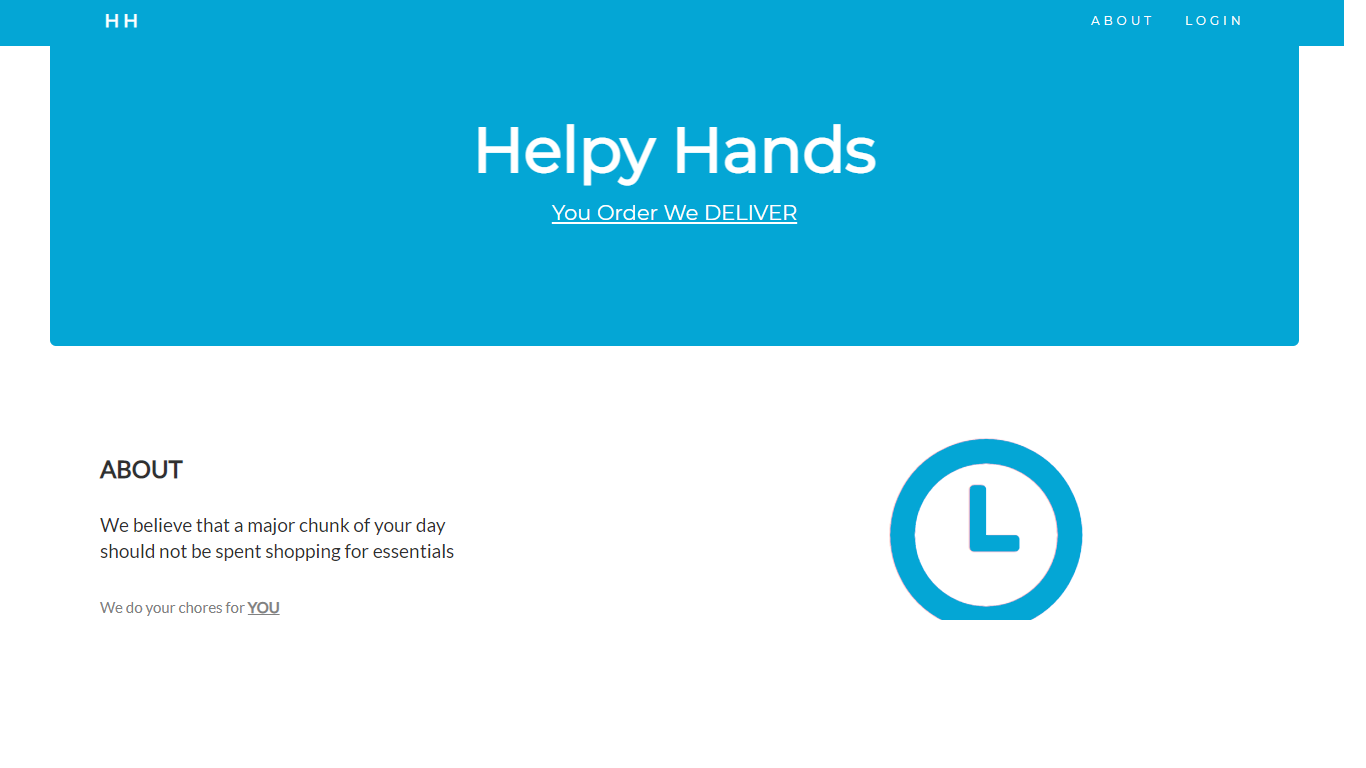
\includegraphics[width=4in,height=1.8in]{../fig/home1}
\caption{Home Page}
\end{figure}\\
\noindent
\begin{figure}[hbtp]
\centering
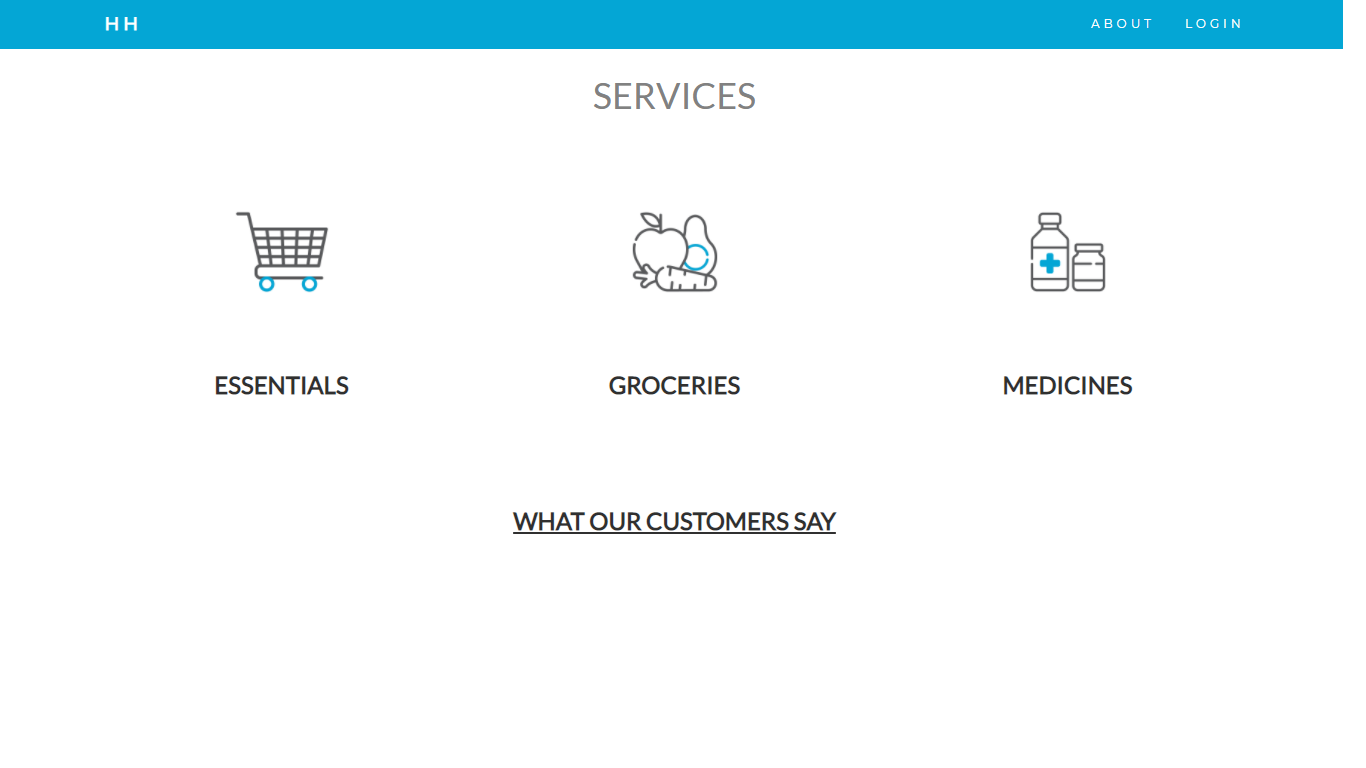
\includegraphics[width=4in,height=1.8in]{../fig/home2}
\caption{Home Page}
\end{figure}\\
\noindent
This is the Helpy Hands home page. It includes the company goals and mission along with a nav link to the login page. The bottom has the customer testimonials reagarding our service.\\
\linebreak
\textbf{Login Page:}\\
\begin{figure}[hbtp]
\centering
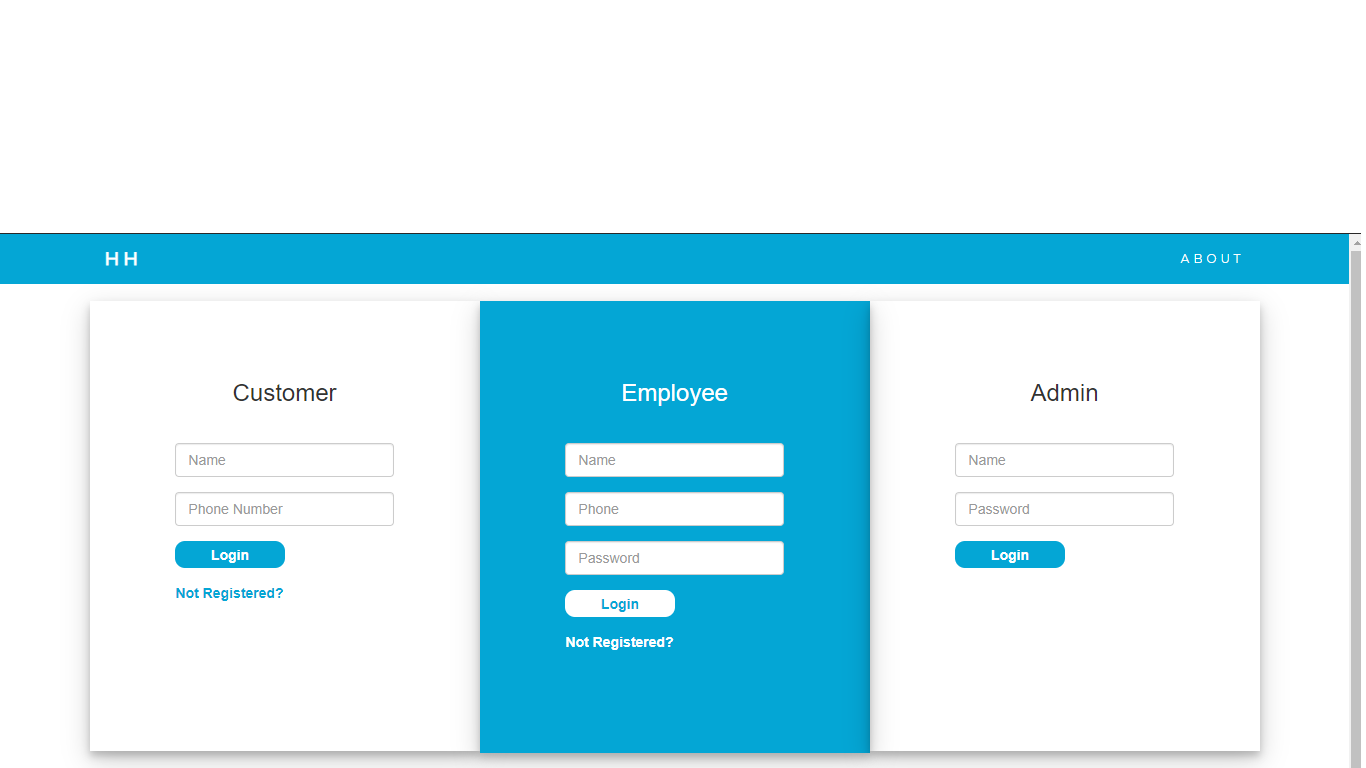
\includegraphics[width=4in,height=1.8in]{../fig/loginpage}
\caption{Login Page}
\end{figure}\\
\noindent
Login form for Employee , Customer and Admin\\
\linebreak
\textbf{Customer Menu}\\
\begin{figure}[hbtp]
\centering
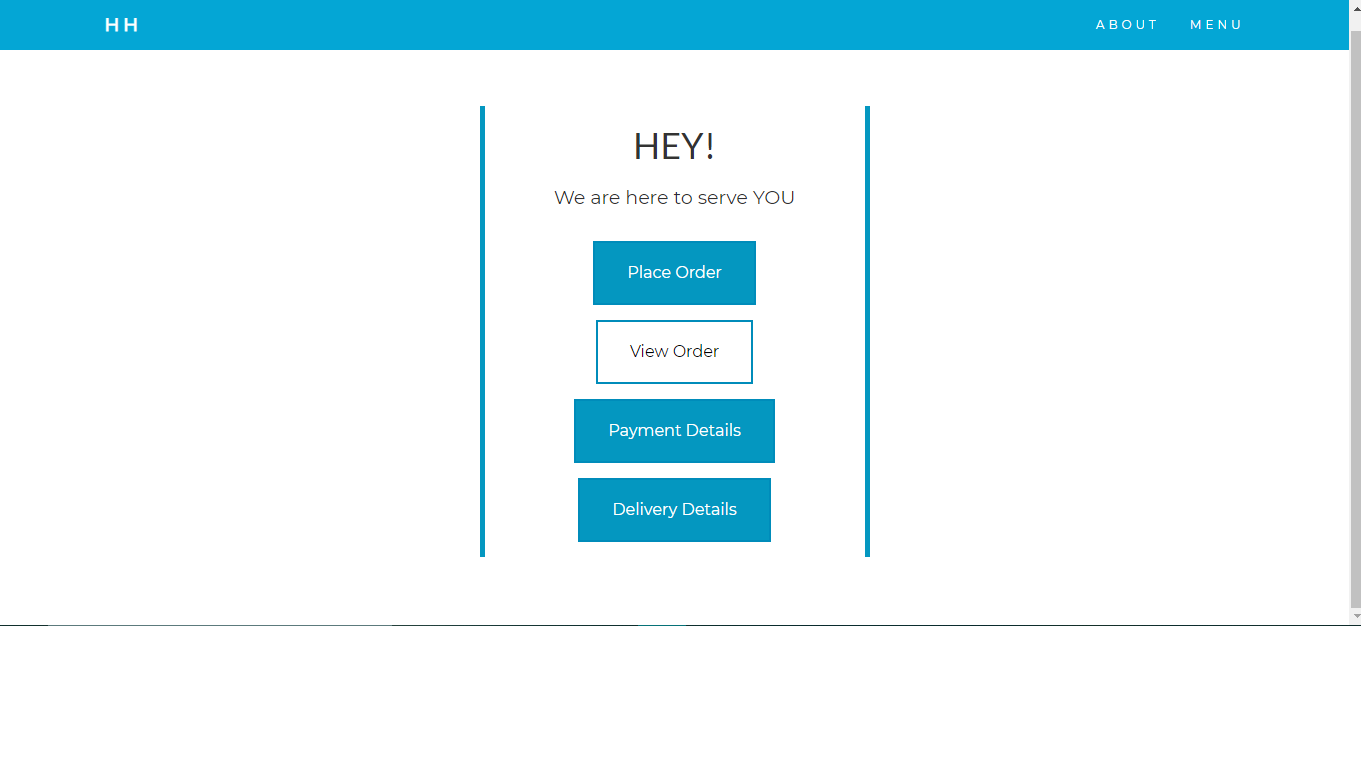
\includegraphics[width=4in,height=1.8in]{../fig/customermenu}
\caption{Customer Menu}
\end{figure}\\
\noindent
This is the customer menu where a customer can place an order or view details of thier orders.\\
\linebreak
\textbf{Employee Menu}\\
\begin{figure}[hbtp]
\centering
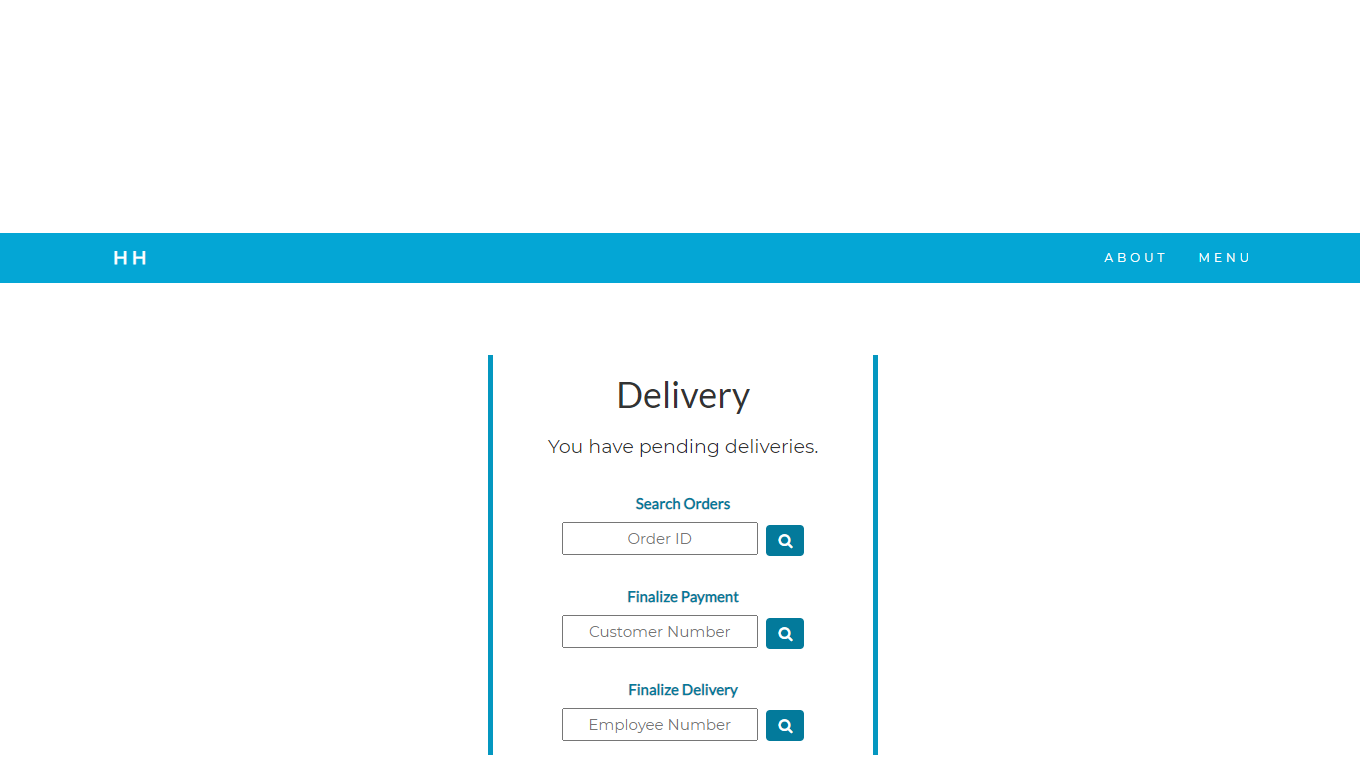
\includegraphics[width=4in,height=1.8in]{../fig/employeemenu}
\caption{Employee Menu}
\end{figure}\\
\noindent
The delivery employee is alerted of his deliveries. The delivery agent can track all details of his deliveries and customers\\
\linebreak
\newpage
\textbf{Admin Menu}\\
\begin{figure}[hbtp]
\centering
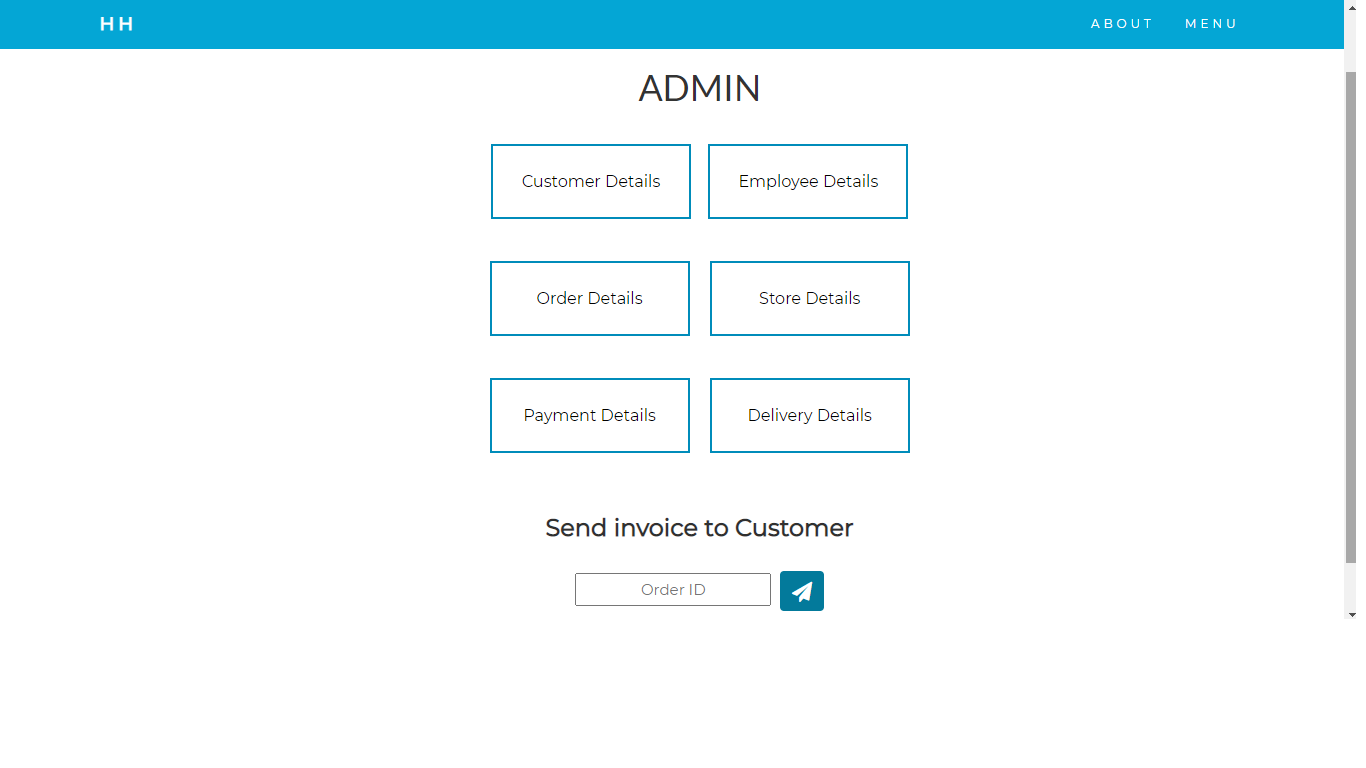
\includegraphics[width=4in,height=1.8in]{../fig/adminmenu}
\caption{Admin Menu}
\end{figure}\\
\noindent
Admin handles the order processing. Admin has master access to everything in the database\\

\chapter{Conclusion and Future work}
\noindent
Helpy Hands Grocery Delivery System will greatly help people from all walks of life. Since we are sometimes too busy or too lazy to go shopping, Having someone do it for us is a life saver.
All supermarkets, vegetable shops, butchers and so on can register themselves as sellers on Helpy Hands and start earning soon after your first sale. Having practically put this idea into action,
We have obtained positive results and looks promising. 
\noindent
Our project can be improved by branching the service into other sectors like , local couriers, medicines and other essentials. Automating the task of the admin willl also improve customer shopping experience
and speed.
Giving a warning when
the product quantity goes low. Keeping a track of the sales that have happened on a particular day,
Issuing gift voucher or discount coupons for the customers.
\newpage
\pagestyle{plain}
\renewcommand{\bibname}{References}
\bibliography{references}
\addcontentsline{toc}{chapter}{References}
\begin{thebibliography}{35}
\bibitem{ds}Database systems Models, Languages, Design and Application Programming, Ramez Elmasri and Shamkant B. Navathe, 6th Edition, Pearson.

\bibitem{dm}Database management systems, Ramakrishnan, and Gehrke, 3rd Edition, 2014, McGraw Hill.

\bibitem{korth}Silberschatz Korth and Sudharshan: Database System Concepts, 6th Edition, Mc-Graw Hill, 2013.

\bibitem{mor}Coronel, Morris, and Rob, Database Principles Fundamentals of Design, Implementation and  
Management, Cengage Learning 2012.

\end{thebibliography}

\end{document}
